%%%%%%%%%%%%%%%%%%%%%%%%%%%%%%%%%%%%%%%%%%%%%%%%%%%%%%%%%%%%%%%%%%%%%
% U.S. ELT KEY SCIENCE PROGRAM DESCRIPTION DOCUMENT ("PROPOSAL")
% Version 1.3, 1 November 2018
%%%%%%%%%%%%%%%%%%%%%%%%%%%%%%%%%%%%%%%%%%%%%%%%%%%%%%%%%%%%%%%%%%%%%

% LaTeX template for writing US ELT Program Key Science Program Description Documents
% (aka "proposals").
% 
% Please fill in all sections.
% 
% The Scientific Justification should be limited to 4 pages including figures (but not including
% references.) There are no strict page limits for other sections, or for the document as a whole, 
% but we suggest a guideline of 8 to 10 pages (excluding cover page and investigators) for the 
% whole document.

%%%%%%%%%%%%%%%%%%%%%%%%%%%%%%%%%%%%%%%%%%%%%%%%%%%%%%%%%%%%%%%%%%%%%

% Please do not modify or delete the following lines.
\documentclass[11pt]{article}
\usepackage{useltp_ksp_1.3}
\usepackage{deluxetable}
\usepackage{natbib}
\begin{document}
\bibliographystyle{aasjournal}

%%%%%%%%%%%%%%%%%%%%%%%%%%%%%%%%%%%%%%%%%%%%%%%%%%%%%%%%%%%%%%%%%%%%%

% SCIENTIFIC CATEGORIES
%
% Please select a scientific category that best describes your
% program by uncommenting only ONE of the selections below.  
% NOTE:  We will probably change this in a future update to allow
% multiple topical areas.

% \sciencecategory{Our Solar System}
% \sciencecategory{Extra-Solar Planetary Systems}
% \sciencecategory{Star and Planet Formation}
% \sciencecategory{Stars and Stellar Evolution}
% \sciencecategory{Resolved Stellar Populations and their Environments}
% \sciencecategory{Galaxy Evolution}
% \sciencecategory{Cosmology and Fundamental Physics}
% \sciencecategory{Astronomical Transients and Multi-Messenger Astrophysics}

%%%%%%%%%%%%%%%%%%%%%%%%%%%%%%%%%%%%%%%%%%%%%%%%%%%%%%%%%%%%%%%%%%%%%%

% TITLE
%
% Give a descriptive title for the proposal in the \title{} command.
%
% Note that a title can be quite long; LaTeX will break the title into
% separate lines automatically.  If you wish to indicate line breaks
% yourself, do so with a `\\' command at the appropriate point in
% the title text.  Use both upper and lower case letters (NOT ALL CAPS).

\title{The Birth and Death of Stars: Initial and Final Mass Functions}

%%%%%%%%%%%%%%%%%%%%%%%%%%%%%%%%%%%%%%%%%%%%%%%%%%%%%%%%%%%%%%%%%%%%%%

% ABSTRACT
%
% Give a general abstract of the scientific justification appropriate
% for a non-specialist.  Write between the \begin{abstract} and 
% \end{abstract} lines.  

% DO NOT remove the \begin{abstract} and \end{abstract} lines.

\begin{abstract}

\end{abstract}

%%%%%%%%%%%%%%%%%%%%%%%%%%%%%%%%%%%%%%%%%%%%%%%%%%%%%%%%%%%%%%%%%%%%%%

% TEAM MEMBER INFORMATION BLOCKS 
%
% Please give names, affiliations, and e-mail addresses of team members here.

% DO NOT remove the \teammembers, \begin{team_member} and \end{team_member} tags.  
% Only one individual's name per \name field is allowed.

\teammembers

\begin{team_member}
\name{Jessica R. Lu}
\affil{UC Berkeley}
\email{jlu.astro@berkeley.edu}
\end{team_member}

\begin{team_member}
\name{Rachel Beaton}
\affil{}
\email{}
\end{team_member}

\begin{team_member}
\name{Tuan Do}
\affil{}
\email{}
\end{team_member}

\begin{team_member}
\name{Dongwon Kim}
\affil{}
\email{}
\end{team_member}

\begin{team_member}
\name{Evan Kirby}
\affil{}
\email{}
\end{team_member}

\begin{team_member}
\name{Michael Meyer}
\affil{University of Michigan}
\email{mrmeyer@umich.edu}
\end{team_member}

\begin{team_member}
\name{Morten Andersen}
\affil{Gemini Observatory}
\email{manderse@gemini.edu}
\end{team_member}

\begin{team_member}
\name{Sukanya Chakrabarti}
\affil{}
\email{}
\end{team_member}

\begin{team_member}
\name{Michael Medford}
\affil{}
\email{}
\end{team_member}

\begin{team_member}
\name{Jennifer Sobeck}
\affil{UW}
\email{jsobeck@uw.edu}
\end{team_member}

\begin{team_member}
\name{Siyao Jia}
\affil{}
\email{}
\end{team_member}
\begin{team_member}

\name{Paolo Turri}
\affil{}
\email{}
\end{team_member}

\begin{team_member}
\name{Fatima Abdurrahman}
\affil{}
\email{}
\end{team_member}

\begin{team_member}
\name{Nicholas Z. Rui}
\affil{}
\email{}
\end{team_member}

\begin{team_member}
\name{Peter Boyle}
\affil{}
\email{}
\end{team_member}

\begin{team_member}
\name{Casey Y. Lam}
\affil{UC Berkeley}
\email{casey$\_$lam@berkeley.edu}
\end{team_member}

\begin{team_member}
\name{Matthew Hosek Jr.}
\affil{UCLA}
\email{mwhosek@astro.ucla.edu}
\end{team_member}

% Duplicate and uncomment the \begin{team_member} to \end{team_member} blocks
% if you have additional team members.   Comment or remove any unneeded blocks.

%%%%%%%%%%%%%%%%%%%%%%%%%%%%%%%%%%%%%%%%%%%%%%%%%%%%%%%%%%%%%%%%%%%%%%
% MAIN PROPOSAL BODY
%%%%%%%%%%%%%%%%%%%%%%%%%%%%%%%%%%%%%%%%%%%%%%%%%%%%%%%%%%%%%%%%%%%%%%

% In the following "essay question" sections, the delimiting pieces of
% markup (\justification, \expdesign, etc.) act as LaTeX \section*{}
% commands.  If the author wanted to have numbered subsections within
% any of these, LaTeX's \subsection could be used.
%
% DO NOT REDUCE THE FONT SIZE, and do not otherwise fiddle with the
% format to get more on a page.  We will reset any changes back to the
% default font.
%
% If you wish to use our "reference" environment, follow the following
% example (journal commands are compatible with AASTeX v4.0):
%
%\begin{references}
%\reference Armandroff \& Massey 1991 \aj, 102, 927.
%\reference Berkhuijsen \& Humphreys 1989 \aap, 214, 68.
%\reference Massey 1993 in Massive Stars: Their Lives in the 
% Interstellar Medium (Review), ed. J. P. Cassinelli and E. B. 
% Churchwell, p. 168.
%\reference Massey \& Armandroff 1999, in prep.
%\end{references}

% PDF figures may be included as follows:
%
% \begin{figure}
%  \begin{center}
%   \includegraphics[width=4.0cm]{sample.pdf}
%   \caption{Sample figure showing important results.}
%  \end{center}
% \end{figure}

%%%%%%%%%%%%%%%%%%%%%%%%%%%%%%%%%%%%%%%%%%%%%%%%%%%%%%%%%%%%%%%%%%%%%%
% PROPOSAL SECTIONS
%%%%%%%%%%%%%%%%%%%%%%%%%%%%%%%%%%%%%%%%%%%%%%%%%%%%%%%%%%%%%%%%%%%%%%

% SCIENTIFIC JUSTIFICATION
%
% Describe the scientific context for this Key Science Program, the specific research question(s)
% to be addressed, and the overall significance to astronomy.  The Scientific Justification 
% should be limited to 4 pages including figures.

\sciencejustification

Stars are a "fundamental particle" for much of astrophysics. While the bulk of stellar evolution is broadly understood, there are two key phases where we have gaping holes in our knowledge: star birth and death. 
At the formation stage, we still lack a predictive model of star formation that can tell us the number and mass of stars that form from a given molecular cloud. 
Observations provide evidence that the outcome of the star formation process -- the initial mass function (IMF) -- is fairly uniform in the local solar neighborhood [REF]; however, there is now evidence that the IMF varies in more extreme environments such as in the Galactic Center \citep{Lu:2013,Hosek:2018} the most massive elliptical galaxies \citep{vanDokkum:2010}, or the least luminous Milky Way satellites \citep{Geha:2013}. 
Mapping variations of the IMF with environment is major observational challenge for the next decade. 
At stellar death, we also lack a predictive model for how a star of a given mass explodes and what kind of remnant it leaves behind. 
This initial-final mass relation depends on the detailed physics of core evolution in the last few hours of a stars life and during the supernovae explosion. 

\section{The Initial Mass Function vs. Environment}
%MA do we want a short statement we will examine disk fractions for the clusters as well? I don't think it's part of the SF science cases (at least not in the JHKLM sense). Perhaps this should go in a star/planet formation science case.

The quest for a predictive theory of star formation, as a function of initial conditions, is far from over.  And almost as important (and frustratingly inseparable) are the properties of multiple systems (companion mass ratio distribution, surface density distribution, and frequency) as a function of primary star mass. 
Most observations reveal a “universal” IMF, and, not surprisingly, many diverse models are able to “explain” it. 
Under intense scrutiny, most claims of detecting a non-universal IMF wither \citep[c.f.][]{Bastian:2010,Luhman:2018}; however there are some unexplained surprises.  
Some of the most persistent, and puzzling, are the claims of bottom-heavy IMFs inferred from various techniques (population synthesis, dynamics, and strong lensing) toward giant elliptical galaxies \citep[e.g.][]{vanDokkum:2010}.  In contrast, two massive young clusters at the Galactic Center appear to be top-heavy \citep{Lu:2013,Hosek:2018b}.
Unfortunately, nearby well-studied star forming regions are poor analogues for diverse star forming events at low metallicity, high pressure, and extreme density which may characterize environments in the early Universe, galactic nuclei, and merger events. 
In order to fully understand the star formation process, the environments of planet formation in their midst, and to support models of galaxy formation and evolution, as well as the chemical evolution, and the frequency of stellar remnants (and stellar mergers) in the Universe over cosmic time, the sensitivity and angular resolution of ELTs is required.
 
In Figure 2, we present a preliminary analysis of how an important nearby star forming region (the Trapezium cluster in the Orion Nebula) would look through AO-assisted imaging on a 6.5 meter telescope (like Magellan) as a function of distance.  
With their 24-30 meter diameter, the ELTs will enable resolution demonstrated [CAN WE GENERALIZE TO TMT+GMT?] below at 25 kpc on a 6.5 meter, but out to 100 kpc!  
Such an observation would be sky background limited at physical radii > 2.5 x that of the star cluster core, enabling direct star counts to measure the IMF down to the hydrogen burning limit in local group galaxies. 
Star formation in the Galactic Center as well as the 
%MA sub-solar metallicity 
LMC and SMC would be dissected with ease. 
The ELTs will also be able to study stellar multiplicity out to several kpc, including several regions of massive star formation.  
%MA extend current studies of the ONC out to several kpc? We will still not get that many close binaries at 2kpc
This will represent a fundamental step in understanding massive star binary properties informing models of core-collapse super nova. 
Recent observations of the R136, a crucial analogue for forming super-star clusters in interacting galaxies, with the SPHERE extreme adaptive optics system on the ESO VLT remain confusion limited in the core (Khorrami et al. 2017 in press - https://arxiv.org/abs/1703.02876). 
Resolving the cores of rich star clusters in the Milky Way and beyond will inform cluster evolution studies and models of black hole formation in their cores for comparison with future gravity wave detections.  
JWST will not help here given its small aperture size. 
To push our understanding of star formation and the IMF to extreme environments where we can hope to put all viable theories to the most stringent tests, requires the angular resolution of the ELTs to overcome the confusion limit. 

\begin{deluxetable}{lccccc}
\tablewidth{0pt}
\tabletypesize{\footnotesize}
\tablecaption{Properties of Young Clusters in Different Environments}
\tablehead{
\colhead{Distance\tablenotemark{a}} & 
\colhead{Cluster Size} & 
\colhead{Stellar Separation} & 
\colhead{Proper Motion} & 
\colhead{Typical Binary} &
\colhead{Hydrogen Burning} \\
\colhead{} &
\colhead{} & 
\colhead{in Core} &
\colhead{for 10 km s$^{-1}$} &
\colhead{Separation} &
\colhead{Limit} \\
\colhead{(kpc)} & 
\colhead{(arcsec)} & 
\colhead{(arcsec)} & 
\colhead{(mas yr$^{-1}$)} & 
\colhead{(mas)} &
\colhead{(K mag)}
} 
\startdata
0.4 (Orion)           & 515.66 & 2.6 & 5.28 & 75.2 & 12.5 \\
8.0 (Galactic Center) & 25.78 & 0.13 & 0.264 & 3.76 & 19.0 \\
60 (LMC)              & 3.44 & 0.02 & 0.035 & 0.50 & 23.5 \\
3500 (M82)            & 0.06 & 3$\times 10^{-4}$ & $6\times 10^{-4}$ & $9\times 10^{-3}$ & 32.0 \\
\enddata
\vspace{-0.1in}
\tablenotetext{a}{Table modified from \citep{Lu:2009}. Cluster size is $\sim$1 pc in diameter. Star separations are based on ONC Trapezium and typical binary separations are $\sim$30 AU.}
\end{deluxetable}

Highlight: North (outer MW, M31) and South (MW, LMC/SMC for low-metallicity, 2 Mpc groups), and all sky (local group galaxies).
%MA Above we note that we can do IMF down to the BD limit at 100kpc, but need the limit at 2Mpc. :

Observational Programs:
Measure IMF in a range of environments:
\textbf{Star Counting:}
Key: Massive Young Clusters, low-metallicity galaxies, etc.  Not only galaxy type but intragalactic environment may influence the IMF -- there is some indication that the outskirts of galaxies (the outer HI disks of galaxies, which are more metal poor and have lower SFR) may have a different IMF from the inner regions of galaxies.  This also has relevance for understanding the host galaxies of LIGO/Virgo sources (Chakrabarti et al. 2017).

Previous observation has shown young stars in the Galactic center have a top-heavy IMF compared to IMF in the solar neighborhood, which indicates an in-situ star formation history. However, this IMF is only derived from the brightest stars (brighter than 15.5 Kp magnitude) in a limited field of view (the central 10’’ within the SMBH in the galactic center). To get a more complete mass coverage for the IMF and determine whether the peak in the IMF also shows any significant difference from nearby star-forming regions, ELT will be perfect to provide deeper spectroscopic observations in a larger field of view (Figure \ref{fig:TMT_YNC}). [see Lu+2013]
-- Siyao		

\begin{figure}
    \centering
    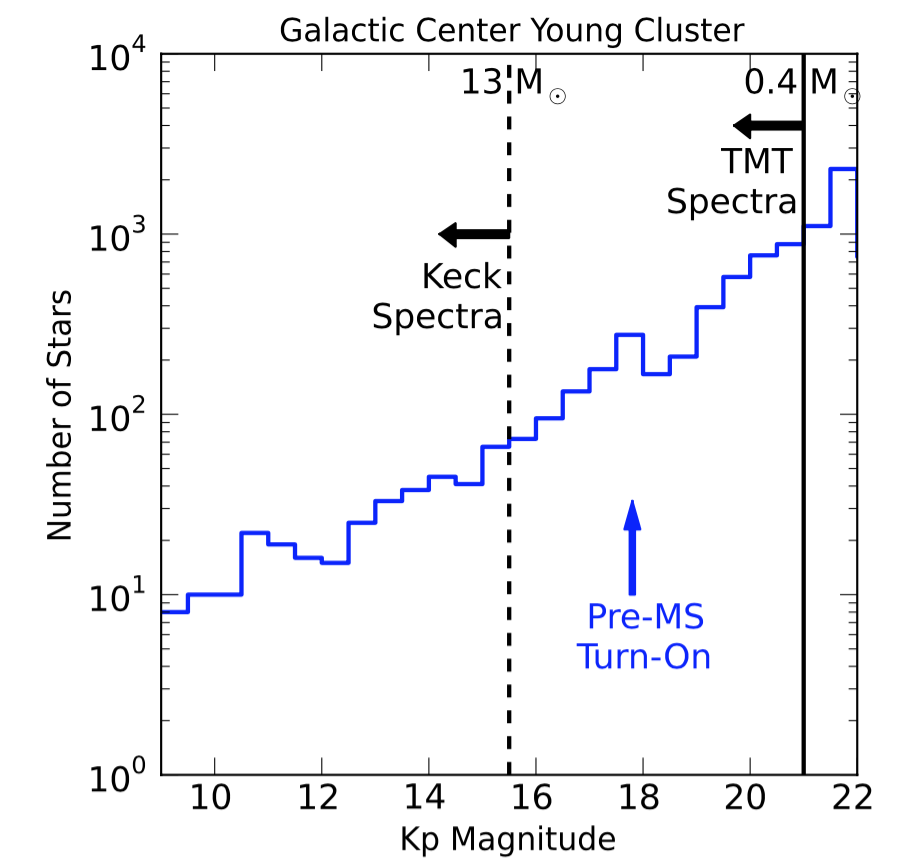
\includegraphics[scale=0.4]{TMT_YNC.png}
    \caption{[NOTE: SCREENSHOT, REPLACE WITH BETTER FIG] Model Kp-band luminosity function for the Young Nuclear Cluster showing the relative sensitivity of Keck spectroscopy (Kp $<$ 15.5 mag) and future TMT+IRIS spectroscopy (Kp $<$ 21 mag). With TMT+IRIS, the pre-main-sequence turn-on point will be detectable at Kp$\sim$17.5 as well as the full IMF shape down to $\sim$0.4 M$_{\odot}$. The model cluster shown here has an IMF slope of 1.7 down to 0.5 M$_{\odot}$ and then turns over at 0.5 M$_{\odot}$ to a slope of 1.3 down to 0.1 M$_{\odot}$ as suggested by [WEIDNER+04] for star formation in the local neighborhood. The model cluster has a distance of 8 kpc and an extinction of AKs = 2.7 mag.
    Figure taken from [LU+13]}
    \label{fig:TMT_YNC}
\end{figure}


Proper motions are a valuable tool for identifying members of stellar clusters. The Young Nuclear cluster at the Galactic Center is incredibly limited by crowding, but a characterization of its stellar population is necessary to explain its anomalous age and constrain its formation scenario. In addition, recent NIR proper motion studies of the Arches cluster have assessed proper motion cluster membership for stars down to $\sim$2.0 solar masses outside of the cluster core (Figure \ref{fig:Arches_cmd}), but the production of a complete proper motion catalog in the cluster core is currently limited by crowding. ELTs’ higher spatial resolution will (1) mitigate the effect of crowding on stellar completeness and (2) provide higher-fidelity proper motions of clusters in the massive core. This allows us to sample the cores of dense, young massive clusters which are differentiated from the extended cluster population photometrically (i.e., by mass segregation) and dynamically.   - Nicholas

\begin{figure}
    \centering
    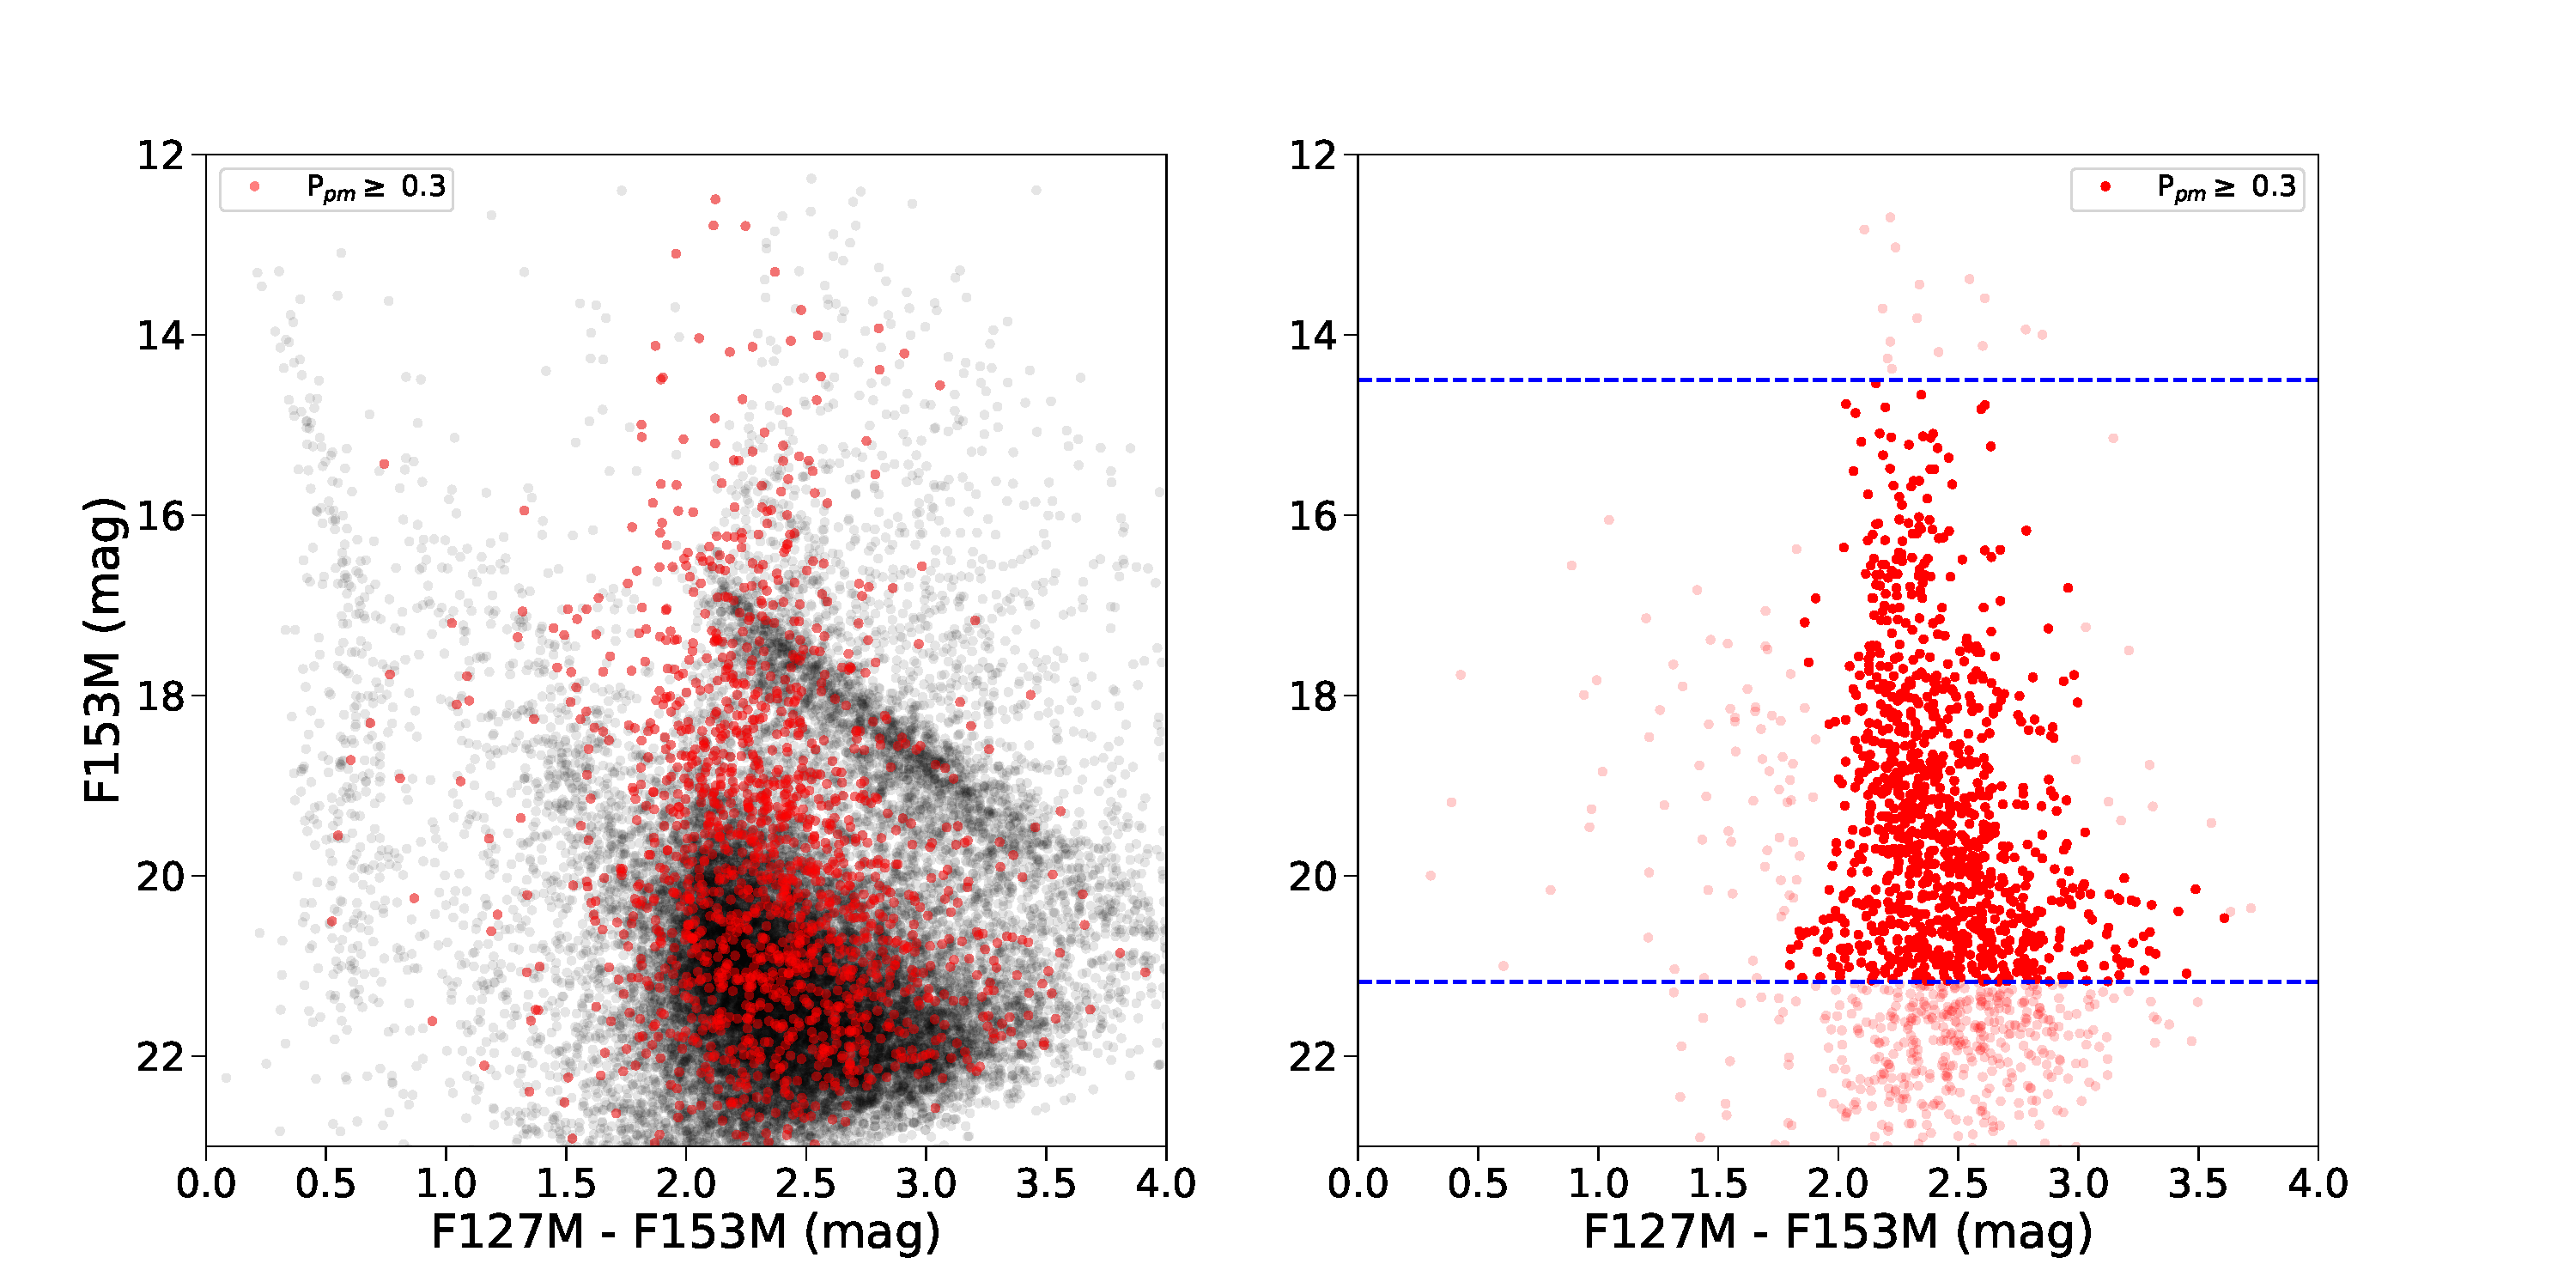
\includegraphics[scale=0.3]{f7.pdf}
    \caption{{\bf Left:} The observed CMD of the Arches Cluster (outside the cluster core, r $>$ 0.25 pc), comparing the proper-motion selected candidate cluster members (red) to the field stars (black). Due to the significant photometric overlap between the populations, proper-motion analysis is required to obtain an accurate cluster sample. {\bf Right:} The differentially de-reddened CMD of candidate cluster members. The sample is at least 30\% complete to F153M = 21.15 mag ($\sim$2 M$_{\odot}$), shown by the fainter blue dotted line. The brighter blue dotted line shows the faint-end boundary of the Wolf-Rayet stars, which are not used in the IMF analysis. The cluster sequence significantly tightens after the differential extinction correction, though a term for residual differential extinction is still required in the IMF analysis.
    Figure taken from [HOSEK+18].}
    \label{fig:Arches_cmd}
\end{figure}

%MA This is not just for the GC; similar problem arises for all clusters in the Galacticmbership disk. The IMF most likely turns over but the field LF keeps rising at fainter magnitudes. Below ~0.2Msun the contamination is higher than cluster members for a lot of the cluster regions. 
The use of adaptive optics on ELTs will provides images and spectroscopy of stellar clusters that are diffraction limited. Because their single apertures will be larger than any optical and infrared telescope currently available, they will have an unprecedented resolution at OIR wavelengths, reducing the confusion and blending of sources in the more crowded environments. One effect will be able to probe the core of most(?) stellar clusters in the Galaxy and to study...        ELTs’ improved resolution lets us count stars in a broader range of environments (confusion-limit in local group). - Paolo

ELTs offer more sensitivity for lower masses, spectroscopy of main-sequence stars in all these clusters (to calibrate mass-magnitude relation). 

ELTs’ can probe clusters at their earliest time and thus the initial stellar distribution 
Mass segregation. Largely a spatial resolution issue hence ELT science - 
The magnitude of mass segregation in star clusters is an important measure that constraints their dynamical evolution histories. To obtain precise mass profiles, high-resolution imaging is required that can handle high crowding and detect low-luminosity stars at the central region of massive clusters. 

\textbf{Integrated Light Spectroscopy}
Key: integrated light from nearby galaxies (this is hard)

\textbf{Star Formation Simulations}
Key: larger clusters, more feedback physics, match environments to observed clusters.

\textbf{Stellar Evolution Models: }
Essential for converting observed properties into masses
ELT can cross-match spectroscopic, photometric, and astrometric observations, allowing for a check on current stellar evolution models and isolated techniques used on previous datasets, eg: matching theoretical isochrone models to photometric analysis of HST data that are lacking spectroscopic confirmation. ELT will constrain photometrically valid models that can then be used on spectroscopically incomplete datasets.

\textbf{Dwarf Galaxies}
One of the extreme environments where IMF variations have been marginally detected is in ultra-faint dwarf galaxies around the Milky Way. One of the limitations in current observations is unresolved background galaxies that overwhelmingly contaminate stellar sources, especially at the lowest masses.  The ELTs increased spatial resolution will completely eliminate issues with star-galaxy separation, allowing IMFs to be estimated all the way down to the hydrogen limit for dozens of ultra-faints (REF Gennaro+ 2018a, 2018b). TO DO: Need to know the distribution of galaxy sizes vs. magnitude... ho w

\section{The Initial-Final Mass Relation}
\begin{itemize}
\item Influences feedback rates (i.e. supernovae types)
\item Need to understand compact object mass functions, binary fractions, kick velocities
\end{itemize}

\begin{figure}
    \centering
    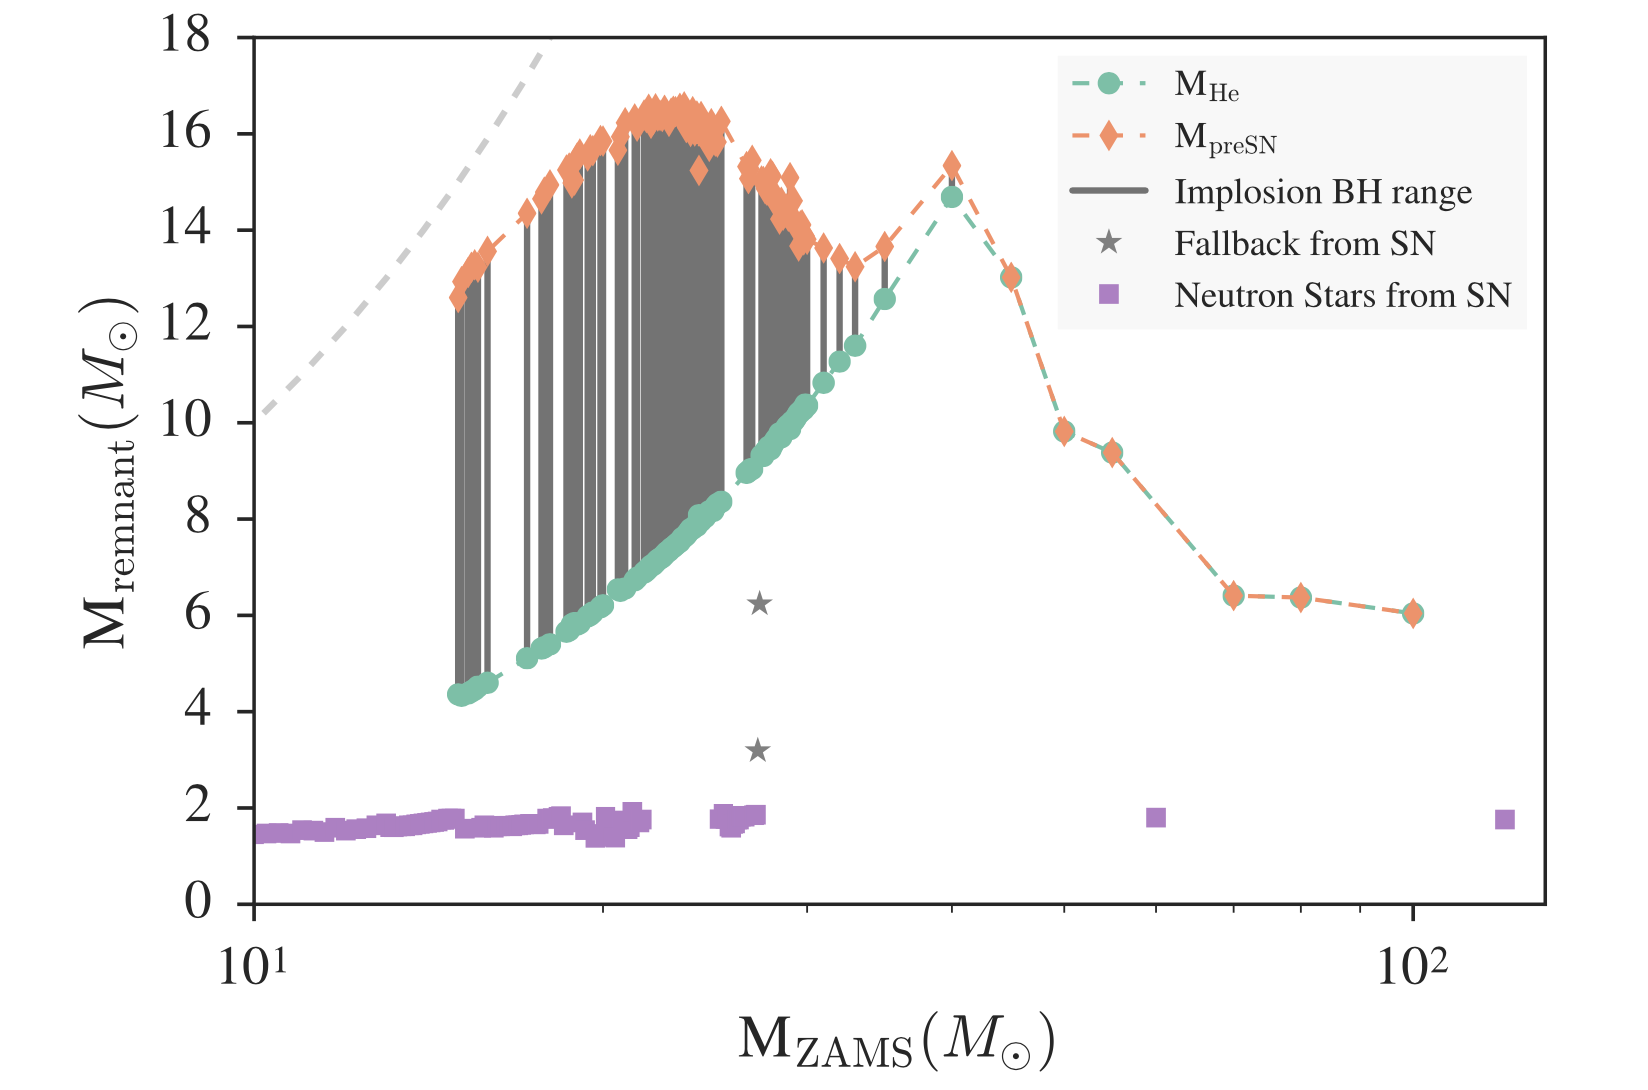
\includegraphics[scale=0.4]{IFMR_raithel.png}
    \caption{IFMR from ``Confronting Models of Massive Star Evolution and Explosions with Remnant Mass Measurements", Raithel, Sukhbold, \"{O}zel 2018, Figure 1.}
\end{figure}

\textbf{Measure IFMR in a range of environments:}
Microlensing to measure masses of a large sample of black holes, neutron stars, and white dwarfs.
Also get stars for free.(didnt mention this point!!)

\textbf{ELTs provide astrometric follow-up to measure masses.}
In order to determine an IFMR once an IMF has been established, it is necessary to measure masses of a large sample of compact objects. One way to circumvent the difficulty of detecting low-luminosity objects such as black holes and neutron stars is to use microlensing. In particular, astrometric microlensing allows for not just the detection of non-luminous objects, but can put constraints on their masses that pure photometric microlensing observations often lack. Currently, the only ground-based telescope capable of an astrometric precision to allow for such detections is Keck, which our team is currently using for astrometric follow-up of candidates discovered in larger microlensing surveys. However, this is only possible to do in the best seeing and weather conditions, and even then is only just precise enough.  The improvement of astrometric precision by a factor of ~3 that ELT would provide allows for astrometric follow-up of dark microlensing candidates to be far more feasible, and would allow for the detection of a sample of compact objects in just a few years.


\textbf{Candidate discovery with all-sky surveys (ZTF, LSST)}
Astrometric microlensing is an expensive measurement and must be undertaken only on those targets already known to be undergoing a microlensing event. Photometric microlensing, or the temporary achromatic amplification of a star’s brightness, is an inexpensive measurement that can be searched for on millions of stars per night. Microlensing surveys to date have focused on observing regions of high stellar density (galactic center, small and large magellanic clouds) to maximize the probability of detecting microlensing events. The next generation of all-sky surveys present the first opportunities to search for microlensing events throughout the galaxy and place meaningful constraints on the nature of gravitational lenses at various galactic latitudes.  The Zwicky Transient Facility (ZTF), a new telescope largely funded through the National Science Foundation's Mid-Scale Innovations Program (MSIP), will generate petabytes of data while conducting a public galactic plane survey in both g and R band filters. These observations strike a balance between areas of the sky with high stellar densities and exploring galactic latitudes not yet observed for microlensing to date. ZTF will generate a near real-time alert stream populated with potential transient candidates found on difference images generated by the telescope. The Large Synoptic Survey Telescope (LSST) will produce an alert stream to the public using the same infrastructure, with an observation cadence and footprint still yet to be determined. Innovative software stacks for extracting valuable science from these alert stream architectures will aid in the discovery of microlensing events for years to come.

\textbf{WFIRST}
Once WFIRST launches, we will move from a regime of detecting 10s of black hole lensing events each year to NNNN events per year. This will dramatically increase the sample of BH lenses with very precise multi-band photometry and simultaneous astrometry. However, WFIRST doesn’t provide continuous coverage of long-duration events because only 40\% of the mission is focused on the microlensing survey and the Galactic Bulge will only be covered for a few months out of the year. The long-duration BH lensing events will likely have incomplete coverage as a result. The next generation of large ground-based telescopes (e.g. TMT and GMT) equipped with adaptive optics systems can provide targeted follow-up during WFIRST gaps. Furthermore, WFIRST is at an L2 orbital position (CHECK) so combining TMT with WFIRST observations will allow us to measure the space-based microlensing parallax that can be combined with the astrometry and photometry to measure the distances to both the lens and source. This will finally allow us to constrain every single parameter for a lensing event, independent of any Galactic model assumption, for a large sample of BH and other compact object lensing events.  Finally, the large ground-based telescopes can provide astrometric measurements for the lowest mass compact objects that WFIRST can’t measure (e.g white dwarfs).  White dwarfs observed today with masses are mostly luminous, more massive, closer, solar metallcity? Can we probe some fainter, lower mass white dwarfs thare of interest? Is that interesting??? 
Also measure their kick velocities, binarity.

\begin{figure}
    \centering
    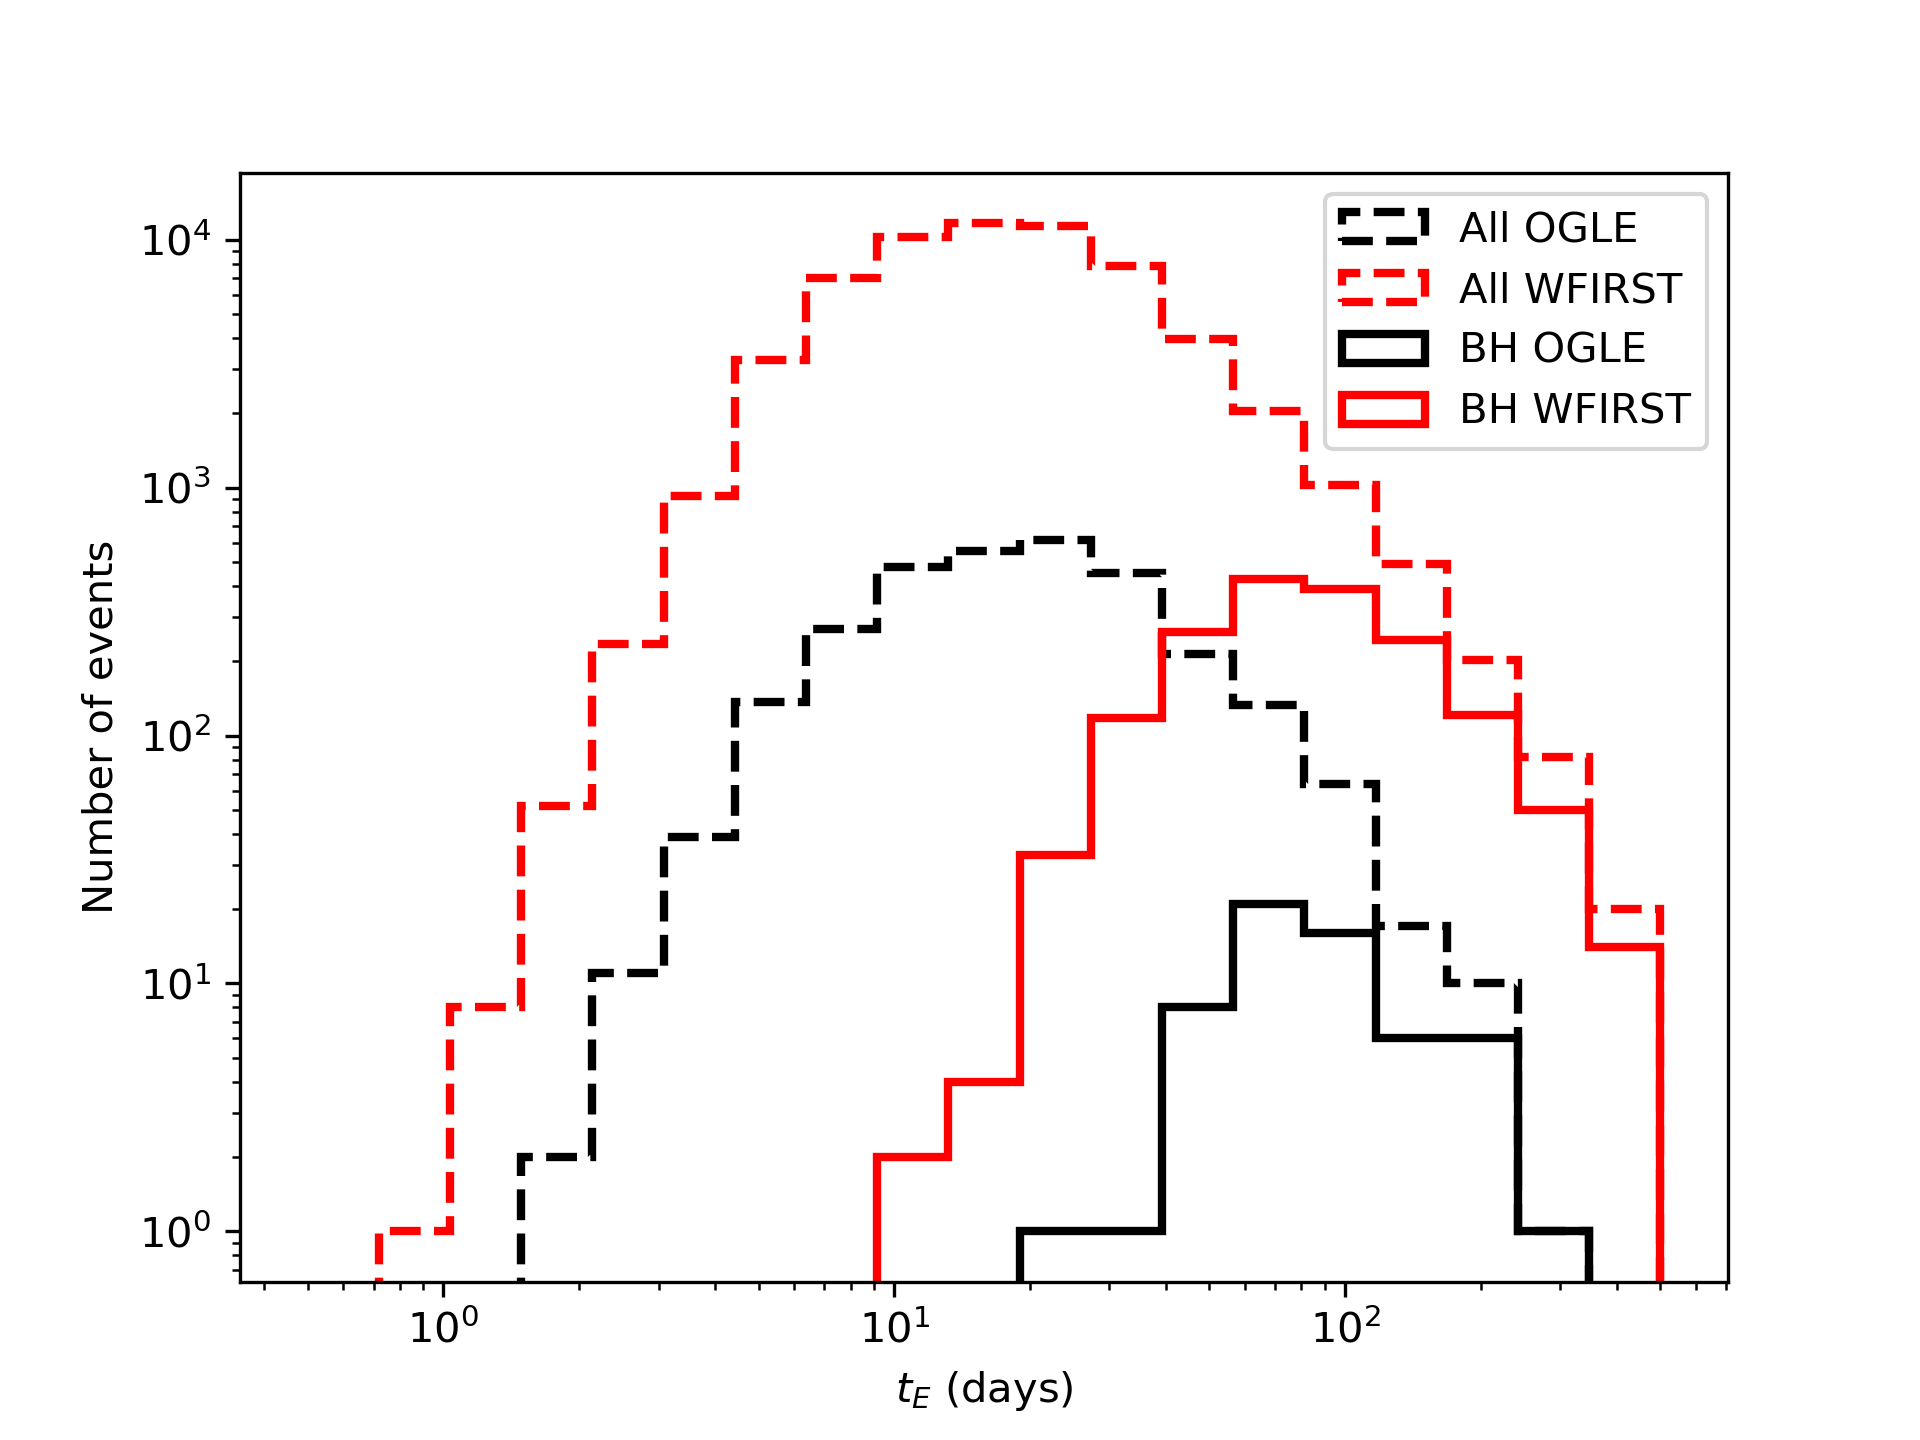
\includegraphics[scale=0.5]{wfirst_v_ogle.png}
    \caption{Number of events seen, WFIRST vs. OGLE. WFIRST will see around 20 times more events overall, and 27 times more BH events than OGLE. The scaling on the y-axis is arbitrary-- identical areas were surveyed for identical durations and with identical cadences ( 4 x 0.34 square degree patches, for 1000 days, at a cadence of 100 days.) The differences are 1) the seeing disks (0.5'' for OGLE, 0.085'' for WFIRST), 2) limiting magnitude (I $< 22$ for OGLE, H $< 26$ for WFIRST). Both of these are constrained to have fblend $>$ 0.1 in their respsective photometric bands, with u0 $<$ 2.}
\end{figure}

\textbf{Search for primordial black holes (this is a tangent)}

UV constraints on the IMF in outer parts of Galaxies. 
Measuring metallicities of outer HI disks could give some expectations of formation of compact objects (massive black holes, neutron stars) in that region. 
Allows GMT \& TMT to act as a single unit 

% TELESCOPES AND INSTRUMENTS
%
% Discuss the program requirements for the telescope(s) (GMT and/or TMT), instrumentation, 
% and adaptive optics systems.  Use of both TMT and GMT in an integrative fashion merits 
% particular attention.  If the program can be carried out using instruments planned for the 
% GMT/TMT early-light suites, discuss what particular capabilities (e.g., spectral resolution, 
% angular resolution, AO performance, etc.) are required.  If new capabilities beyond the 
% defined early-light instruments are needed, describe the requirements in a suitable level 
% of detail.


\telinstreq

% EXPERIMENTAL DESIGN
%
% Describe the details of the observational program, including:
%  o Target/sample selection.  This may be a description of a target selection strategy that would be
%    appropriate in the future when the project would be executed. Specific targets may be specified,
%    particularly if they demonstrate the value of a 2-telescope, 2-hemisphere system.
%  o A description of the required observations.
%  o Signal-to-noise requirements and exposure time estimates.  Because the detailed parameters of future
%    instruments may not be precisely known now, this section should discuss the assumptions adopted.
%  o Special requirements for observing conditions (if appropriate), in particular with regard to
%    image quality and adaptive optics, precipitable water vapor, or other special conditions.
%  o Scheduling requirements (as appropriate), including lunar phase, observing cadence,
%    and/or timing constraints.

\expdesign

% OBSERVING PROGRAM SUMMARY
%
% Summarize the overall observing program.  This should include:
%  o A high-level review of the program as it would be executed, potentially over several years,
%    including the sequence of observations if relevant.
%  o The total observing time required for each telescope, instrument, and instrument mode used,
%    based on the detailed information from the Experimental Design.

\obssum

% LEGACY VALUE
%
% Discuss the legacy value of these observations and the data they would generate for the broader 
% scientific community, including a description of potential data products and the ancillary 
% science that might be enabled by this dataset.

\legacyvalue

% ANALYSIS PLAN
%
% Describe the program requirements for data analysis and interpretation.  This may include:
%  o Data management and software needed for data reduction and analysis.
%  o Simulations needed to interpret the data.
%  o Other resources (e.g., computational, user support) that may be necessary.

\analysisplan

% SYNERGY WITH OTHER FACILITIES OR RESOURCES
%
% If relevant, describe how the proposed TMT/GMT observations complement data from other facilities. 
% This may include:
%  o Required coordination between the proposed GMT/TMT program and observations or data resources
%    from other facilities in space or on the ground.
%  o Preparatory or ancillary datasets that will be required to carry out this Key Science Program.

\otherfacilities

%%%%%%%%%%%%%%%%%%%%%%%%%%%%%%%%%%%%%%%%%%%%%%%%%%%%%%%%%%%%%%%%%%
\bibliography{imf_ifmr}
% Please do not modify or delete this line.
\end{document}

%%%%%%%%%%%%%%%%%%%%%%%%%%%%%%%%%%%%%%%%%%%%%%%%%%%%%%%%%%%%%%%%%%
